\scanpage{20}

\fbox{Lemmes sur coeff. binomiaux}

\figure{\begin{tikzpicture}\draw (0,0)--(0,-5);\end{tikzpicture}}
\uline{Lemme 1} Soient $p$ nb premier, $i,j\in\mathbb N$, avec un développement $p$-adique
\[
i=\sum_{0\leq\varepsilon\leq\unsure{e}}u_\varepsilon p^\varepsilon\qquad
j=\sum_{0\leq\varepsilon\leq\unsure{e}}v_\varepsilon p^\varepsilon\qquad
0\leq u_\varepsilon,v_\varepsilon\leq p-1,
\]
soit
\[
c_{ij}=\frac{(i+j)!}{i!\,j!}\in\mathbb Z\qquad(\text{coeff. binômial})
\]
alors on a
\[
c_{ij}\not\equiv0\ (p)\quad\text{sss}\quad u_\varepsilon+v_\varepsilon\leq p-1\quad\forall\varepsilon\quad(0\leq\varepsilon\leq\nu)
\]
et \deleted{pour} on a en tous cas
\[
c_{ij}\equiv\prod_{0\leq\varepsilon\leq\nu}c_{u_\varepsilon,v_\varepsilon}\qquad(p)
\]

\margin{\uline{\unsure{Cor!|Car!}}}
\figure{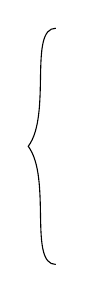
\begin{tikzpicture}\draw (0.35,0) .. controls (0,0) and (0.3,-1.1) .. (0,-1.5) .. controls (0.3,-1.9) and (0,-3) .. (0.35,-3);\end{tikzpicture}}
On écrit \unsure{d'abd.}
\[
i=u+pr,\quad j=v+ps\qquad0\leq u,v\leq p-1,\quad r,s\geq0
\]
et on montre que
\[
(*)\quad\begin{cases}
c_{ij}\not\equiv0\ (p)\quad\text{sss}\quad u+v\leq p-1\text{ et }c_{r,s}\not\equiv0\ (p)\\
c_{ij}\equiv c_{u,v}\,c_{r,s}\qquad(p)
\end{cases}
\]
en étudiant le développement, dans $\mathbb F_p[X,Y]$, de $(X+Y)^{i+j}$. \deleted{\unsure{On}} a
\[
i+j=p\underbrace{(r+s)}_t+\underbrace{u+v}_{\deleted{\unsure{v}}\inserted{w}}
\]
si $w\leq p-1$ on écrit
\[
\begin{aligned}
(X+Y)^{i+j}&=((X+Y)^p)^{\unsure{t}}(X+Y)^w=(X^p+Y^p)^{\unsure{t}}(X+Y)^w\\
&=\sum_{\substack{0\leq\alpha\leq w\\0\leq\beta\leq t}}\binom{w}{\alpha}\binom{t}{\beta}X^{\alpha+p\beta}Y^{(w-\alpha)+p(t-\beta)},
\end{aligned}
\]
où tous les monômes écrits dans la somme sont à exposants distincts. On a donc comme coeff. de $X^iY^j$ celui correspondant au terme $i=\alpha+p\beta$ i.e.
\[
\alpha=u,\quad\beta=r\qquad\text{i.e.}
\]
\[
c_{i,j}\equiv\binom{w}{u}\binom{t}{r}=c_{u,v}\,c_{r,s}\qquad(p)
\]
et il est immédiat que $c_{u,v}\not\equiv0\ (p)$, car $c_{u,v}=\dfrac{(u+v)!}{u!\,v!}$
\[
0\leq u,v,u+v\leq p-1.\qquad\text{Donc}\quad c_{ij}\not\equiv0\ (p)\Longleftrightarrow c_{r,s}\not\equiv0\ (p).
\]
Il reste à voir que si $w\geq p$, \deleted{soit $w=p+w'$} \inserted{alors} $c_{i,j}\equiv0\ (p)$
\[
\text{Soit }\unsure{w'|w}=p+w'\qquad0\leq w'\leq p-2,\quad\text{donc}\quad
\inserted{i+j=(r+s+1)p+w'=\underbrace{(t+1)}_{t'}p+w',}
\]
\[
(X+Y)^{i+j}=(X^p+Y^p)^{\unsure{t'}}(X+Y)^{w'}
=\sum_{\substack{0\leq\alpha\leq w'\\0\leq\beta\leq t'}}\binom{w'}{\alpha}\binom{t'}{\beta}X^{\alpha+\beta p}Y^{(w'-\alpha)+p(t'-\beta)}.
\]
\unsure{Trouver} un $X^iY^j$ correspondant à $\alpha=u,\beta=r$, il faudrait $u=\alpha\leq w'=u+v-p$ donc $v\geq p$, ce qui n'est pas, donc il n'y a pas de

\mspage{19}
